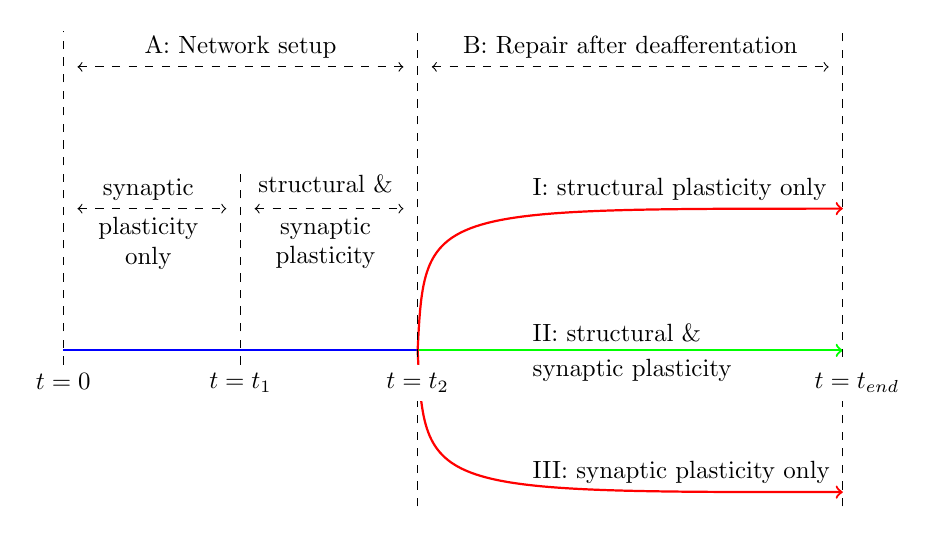
\begin{tikzpicture}[scale=0.9, transform shape]

  % horizontal lines
  \draw[blue, thick] (0,4) -- (5,4);
  \draw[green, thick, ->] (5,4) -- (11,4);
  \draw[red, thick, ->] (5,4) .. controls (5.1,6) .. (11,6);
  \draw[red, thick, ->] (5,4) .. controls (5.1,2) .. (11,2);


  \draw[dashed] (0,3.8) -- (0,8.5);
  \node[below] at (0, 3.8)  {\(t=0\)};

  \draw[dashed] (2.5,3.8) -- (2.5,6.5);
  \node[below] at (2.5, 3.8)  {\(t=t_1\)};

  \draw[dashed, -] (5,1.8) -- (5,8.5);
  \node[below, fill=white] at (5, 3.8)  {\(t=t_2\)};

  \draw[dashed] (11,1.8) -- (11,8.5);
  \node[below, fill=white] at (11.2, 3.8)  {\(t=t_{end}\)};

  \draw[dashed, <->] (0.2,8) -- (4.8,8);
  \node[above] at (2.5,8) {A: Network setup};

  \draw[dashed, <->] (0.2,6) -- (2.3,6);
  \node[above] at (1.2,6) {synaptic};
  \node[below, align=center] at (1.2,6) {plasticity\\only};
  \draw[dashed, <->] (2.7,6) -- (4.8,6);
  \node[above] at (3.7,6.1) {structural \&};
  \node[below, align=center] at (3.7,6) {synaptic\\plasticity};

  \draw[dashed, <->] (5.2,8) -- (10.8,8);
  \node[above] at (8,8) {B: Repair after deafferentation};


  \node[above right, align=left] at (6.5,6) {I: structural plasticity only};
  \node[above right, align=left] at (6.5,4) {II: structural \&};
  \node[below right, align=left] at (6.5,4) {synaptic plasticity};
  \node[above right, align=left] at (6.5,2) {III: synaptic plasticity only};

\end{tikzpicture}
